\documentclass[12pt,twoside,titlepage]{ingenius}
\usepackage[figuresright]{rotating}
\usepackage{pgfplots} 
\pgfplotsset{compat=1.7}
\usepackage{adjustbox}
\usepackage{units}
\usepackage{dblfloatfix}
\usepackage{amssymb}
\usepackage{caption}
\usepackage{subcaption}
\usepackage{bm}
\usepackage{textcomp}
\usepackage{pifont}
\usepackage{cite}
\usepackage{xcolor,colortbl}
\usepackage{amsmath}
\usepackage{upgreek}
\usepackage{graphicx}
\usepackage{tikz}%flujogramas
\usepackage{pifont}
\usetikzlibrary{shapes,arrows}
\usepackage{textcomp}
\usepackage{multirow}
\usepackage{float}
\usepackage{soul}
\usepackage{rotating}
\usepackage{hyperref}
\usepackage{booktabs}
\usepackage{algorithmic}
\usepackage[ruled,vlined,algo2e]{algorithm2e}
\usepackage{algorithm}
%\usepackage{fancyhdr}
%\pagestyle{fancy}
\makeatletter
\renewcommand*{\ALG@name}{Algoritmo}
\makeatother
\graphicspath{{figures/}}
%===========================================
%========
\usepackage{tikz,xcolor,hyperref}
% Make Orcid icon
\definecolor{lime}{HTML}{A6CE39}
\DeclareRobustCommand{\orcidicon}{%
	\begin{tikzpicture}
	\draw[lime, fill=lime] (0,0) 
	circle [radius=0.16] 
	node[white] {{\fontfamily{qag}\selectfont \tiny ID}};
	\draw[white, fill=white] (-0.0625,0.095) 
	circle [radius=0.007];
	\end{tikzpicture}
	\hspace{-2mm}
}
\foreach \x in {A, ..., Z}{%
	\expandafter\xdef\csname orcid\x\endcsname{\noexpand\href{https://orcid.org/\csname orcidauthor\x\endcsname}{\noexpand\orcidicon}}
}
%========================================================
\titulo{Título de artículo en Español}
\tituloa{Article title in English}
%========================================================
\newcommand{\orcidauthorA}{0000-0002-7645-8793}
\newcommand{\orcidauthorB}{0000-0002-0837-0642}
\newcommand{\orcidauthorC}{0000-0002-4704-1067}
\autores{Nombre Autor $^{1}$,\orcidA{}, Nombre Autor $^{2}$,\orcidB{}, Nombre Autor$^{3}$,\orcidC{}}
\adscripcionautor{%
$^{1}$ En esta sección escriba la adscripción institucional actual en el siguiente orden: Dependencia a la que pertenece en su institución, Institución a la que pertenece,  país.\\
$^{2}$Laboratorio de Investigación en Sistemas Informáticos e Inteligencia Artificial, Universidad Politécnica de Valencia - España.\\
$^{3}$ Autor 3, Dependencia, Institución, Ciudad, País, e-mail: correoelectrónico@autorparacorrespondencia}

%%Datos para referencias
\newcommand{\apellido}{Apellido autor et al.}% Apellido o apellidos para referencia 
\newcommand{\titu}{Titulo del articulo}%titulo a la ref\erencia
\newcommand{\tipo}{Art\'iculo Cient\'if{}ico / Scientif{}ic Paper} 
%tipo de documento Punto de vista/Point of view,  Art\'iculo Cient\'if{}ico / Scientif{}ic Paper, Rese\~na bibliogr\'afica/Review
%========================================================
%%Datos para propiedades del pdf no requiere ser llenado
\newcommand{\autor}{}%autor para propiedades del pdf
\newcommand{\pc}{}%palabras clave para propiedades del pdf
\newcommand{\kw}{}%keywords para propiedades del pdf
\usepackage{xcolor}
\usepackage{color}
\usepackage{titlesec}
\usepackage[spanish,english]{babel}
\titleformat{\section}
{\large \bfseries }
{\thesection.}{.5em}{}

\titleformat{\subsection}
{\normalsize \bfseries  }
{\thesubsection.}{.5em}{}

\titleformat{\subsubsection}
{\normalsize \bfseries }
{\thesubsubsection.}{.5em}{}

\usepackage{fancyhdr}
\pagestyle{fancy}
\fancyhf{}
\fancyhead[LO]{} % En las páginas impares, parte izquierda del encabezado, aparecerá el nombre de capítulo
%\fancyhead[RE]{{\rule[-2ex]{0pt}{3ex} \bf \revista} N.$^\circ$ \num, \mest \, de \anoc} % En las páginas pares, parte derecha del encabezado, aparecerá el nombre de sección
\fancyhead[LE,RO]{ \large \thepage  } % Números de página en las esquinas de los encabezados
\fancyhead[LO]{\rule[-2ex]{0pt}{3ex} {\it \apellido \,/ \titu}} % Números de página en las esquinas de los encabezados
%\fancyfoot[LE,RO]{\thepage} %Escribo este texto a la izquierda en las páginas impares y a la derecha en las pares
%\fancyfoot[LO,RE]{ \rule{300pt}{0.5pt}\\ \textsc{Ingenius}, {\it  Revista de Ciencia y Tecnolog\'ia.}\\ \copyright  \, 2013, {Universidad Polit\'ecnica Salesiana, Ecuador.}} %Escribo este texto a la izquierda en las páginas impares y a la derecha en las pares
%\fancyfoot[LO,RE]{\textsc{Ingenius}, {\it  Revista de Ciencia y Tecnolog\'ia}, 7(1) 2012: 1-6. \\ \copyright  \, 2012, {Universidad Polit\'ecnica Salesiana, Ecuador.}} %Escribo este texto a la izquierda en las páginas impares y a la derecha en las pares
\renewcommand{\headrulewidth}{0.5pt}
%\renewcommand{\footrulewidth}{0.5pt}

\usepackage[]{hyperref}
\hypersetup{
    pdftitle={\titu},
    pdfauthor={\autor},
    pdfsubject={Ingenius -- Revista de Ciencia y Tecnolog\'ia},
    pdfkeywords={\pc; \kw},
    pdfborder={0 0 0},
   % bookmarks=true,
pdfstartpage=1,
pdfproducer=pdf\TeX{}-1.40.13. 
}



\usepackage{xcolor}
\usepackage{color}
\usepackage{listings}%% lista de códigos
\usepackage{tikz}
%\input{config_c}
\usepackage{listings}%% lista de códigos
	\lstset{ 
		linewidth=0.5\textwidth,
		frame=tb,	
		%framerule=0.5pt,
		aboveskip=0.5cm,%Distancia Texto al codigo
		%framextopmargin=3pt,%Distancia Primera Linea-Borde Superior
		framexbottommargin=3pt,%Distancia Ultima Linea-Borde Inferior
		%framexleftmargin=0.4cm,%Distancia Borde Izquierdo Codigo-Borde Izquierdo Pagina
		framesep=0pt,
		rulesep=.8pt,%Espesor linea junto a los numeros
		backgroundcolor=\color{gray!10},
                     numbersep=5pt,
                     xleftmargin=3pt,
                     xrightmargin=8.5pt,
                     framextopmargin=10pt,
		rulesepcolor=\color{black},
		stringstyle=\ttfamily,
		floatplacement=htb,
		boxpos={c},
		breaklines=true,
		breakatwhitespace=true,
		showstringspaces = false,
		basicstyle=\small\ttfamily,
		commentstyle=\color{gray!45},
		keywordstyle=\bfseries,
		%linewidth=0.8\textwidth,
		title=\lstname,
		%numbers=right,%Posicion de los Numeros left=izquierda; right=derecha
		%numbersep=15pt, %separacion de numero 1,2,3,4 hacia el frame
		numberstyle=\tiny,
		numberfirstline = false,
		breaklines=true,
		}
	\lstnewenvironment{listing}[1][]
		{\lstset{#1}\pagebreak[0]}{\pagebreak[0]}
		\lstdefinestyle{consola}
		{basicstyle=\scriptsize\bf\ttfamily,
		 backgroundcolor=\color{gray75},
		}
	\lstdefinestyle{C}
		{language=C,
}

\newenvironment{tabla}
  {\par\bigskip\noindent\minipage{\linewidth}}
  {\endminipage\par\bigskip}

\newenvironment{figura}
  {\par\bigskip\noindent\minipage{\linewidth}}
  {\endminipage\par\bigskip}

\newenvironment{pseudo}
  {\par\noindent\minipage{\linewidth}}
  {\endminipage\par\bigskip}
%========================================================
\begin{document}
\renewcommand{\lstlistingname}{Algorithm}
\setcounter{page}{1}
\renewcommand{\refname}{Referencias}
\renewcommand{\figurename}{Figura}
\renewcommand{\tablename}{Tabla}
\frenchspacing

\begin{tikzpicture}[overlay]
  \node at (138.5mm,12.2mm){
\includegraphics[scale=0.35]{figures/logoingenius.pdf}};
 \node at (138mm,2mm){\textsf{\scriptsize pISSN: 1390-650X / eISSN: 1390-860X}};
   \node at (79mm,10mm){
\includegraphics[scale=0.6]{figures/creativec.pdf}};
\end{tikzpicture}

\input{silabeo}
\membrete
\input{configuracion_portada}

%\begin{textblock}{12.4}(0,10)
\begin{textblock}{12.4}(0,10)%Modificar Editor Ingenius cuando se inserte Creative Commons
\adscripcion
\end{textblock}
%========================================================
\begin{table}[htb]
\begin{tabular}{p{8cm}p{8cm}}
{\Large \bfseries Resumen} &{\Large \bfseries Abstract} \\ \\
En este documento se encuentran detallas las instrucciones para preparar un artículo para la Revista de Ciencia y Tecnología INGENIUS y puede emplearse como plantilla. Se presenta el formato de publicación, además contiene las normas para presentar ecuaciones, figuras, tablas y referencias.  Los autores deben seguir las instrucciones para mantener el estándar de publicación. Como habrá notado, esta primera sección es para generar un resumen del contenido del artículo dando una clara indicación del objetivo, alcance y los principales resultados para que los lectores puedan determinar si el texto completo será de su particular interés. Debe contener un máximo de 230 palabras, no debe incluir ecuaciones o referencias. El contenido del resumen debe estar completamente justificado. 

&Redactar aquí el resumen en inglés con las mismas especificaciones del formato descrito en resumen.
……………..
\\[-0.3cm]
\palabrasclave{Incluya aquí las palabras claves que tienen relación con el contenido o enfoque del artículo. Las palabras clave serán de tres a seis, se citarán en orden alfabético y separadas por comas.}&\keywords{Escriba nuevamente las palabras claves en inglés.}  \\
\end{tabular}
\end{table}

\newpage

\begin{multicols}{2}
%========================================================
\section{Introducción}
\vspace{-0.15cm}

Este documento es una plantilla de \LaTeX~ para la preparación de artículos. Incluye: descripción, espaciados e información relacionada para generar la versión final de los artículos a publicarse en la Revista INGENIUS. 
 
Si es necesario puede consultar las Normas para la publicación de artículos disponible en el enlace  \url{https://bit.ly/2Pq94C6}. 
Siga cuidadosamente estas indicaciones y en caso de alguna duda puede escribir a la dirección de correo revistaingenius@ups.edu.ec.

\subsection{Instrucciones para preparar manuscritos}

La revista INGENIUS publica resultados de investigación sobre desarrollo, informes, estudios y propuestas así como revisiones de literatura (state of the art). Los trabajos deben ser originales, no haber sido publicados en ningún medio ni estar en proceso de arbitraje o publicación. De esta manera, las aportaciones en la revista pueden ser:

\begin{itemize}
\item \textbf{Investigaciones, informes, estudios y propuestas:} deben tener de 5000 a 6000 palabras
\item \textbf{Revisiones del estado del arte:} deben tener de 6000 a 7000 palabras.
\end{itemize}

La cantidad de palabras incluyen títulos, autores, adscripción institucional,  resúmenes, palabras clave, tablas y referencias. En las Revisiones del estado del arte es importante tener referencias bibliográficas de alrededor unas 40 obras de preferencia actuales.

Los artículos deben seguir la estructura IMRDC:

\begin{itemize}
    \item Introducción
    \item Materiales y Métodos
    \item Resultados y Discusión
    \item Conclusiones
\end{itemize}

En todas las tipologías de trabajos son obligatorias las Referencias Bibliográficas. Los Agradecimientos y Notas serán opcionales y deberán ir al final del artículo (antes de las referencias), para mayor información consultar las Nomas de publicación de artículos en: \url{https://bit.ly/2Pq94C6}.

La versión final del artículo se debe enviar en un archivo en formato PDF conjuntamente con un archivo comprimido del archivo fuente de overleaf.

\section{Materiales y Métodos}

Las secciones de Introducción, Materiales y Métodos, Resultados y Discusión y Conclusiones del artículo pueden estructurarse divididas en diferente forma. En cada epígrafe del artículo se deben enumerar como máximo hasta tres niveles: 1. / 1.1. / 1.1.1. En esta plantilla en la sección materiales y métodos se explica cada una de las partes del manuscrito y como elaborarlo.

\subsection{Título principal}

El título principal (en la primera página) debe estar centrado, se debe respetar el codigo establecido para el efecto, respetando además el orden de mayusculas y minusculas, ya que el mismo se mostrará después de la compilación con la tipografía de fuente \textsc{Versalitas}.

\subsection{Nombre del Autor(s) y afiliaciones}

Los nombres del autor(es) deben estar centrados abajo del título y deben ser ingresados en el código indicado, tal como se indica en la parte superior de este documento.
      Se escribirá primero el nombre y luego el apellido. En el caso de que el artículo tenga más de un autor, los nombres estarán separados por comas de manera que todos los nombres se los autores estén en una sola línea. Los detalles de los autores no deben mostrar ningún título profesional como PhD, MSc, Dr.

\subsection{Títulos de primer, segundo y tercer nivel}

El primer nivel corresponde al título principal de cada epígrafe, use el comando "\emph{section}", se debe usar un punto después del número del título.

El segundo nivel corresponde a los subtitulos use el comando "\emph{subsection}"; mientras que para los subtitulos de tercer nivel use el comando "\emph{subsubsection}" 

La configuración de esta plantilla permitirá que en cada nivel se muestre el tamaño de texto que identifique a cada uno.

\subsection{Texto principal}

El texto principal del artículo deberá ser colocado respetando las reglas gramaticales la condiguración de la plantilla mostrará los espaciados, tipo de fuente, sangrías, etc.

\subsection{Figuras, tablas, ecuaciones, unidades y abreviaturas.}

Figuras: Todas las figuras deben estar cargadas en la carpeta del código fuente denominada "\emph{figures}" con un nombre caracteristico que identifique a cada figura que conste en el artículo, utilice el código a continuación indicado para llamar a cada figura según corresponda en el texto del artículo, de la misma manera en el campo "\emph{caption}" colocar el nombre de la figura. Las figuras pueden estar en formato .jpg .png o .pdf con una resolución mínima de 300 dpi (ver Figura \ref{figura1}). También se pueden insertar código para figuras que usen el paquete TiKz o Pgfplots como muestra la Figura \ref{figura2}. Todas las figuras deben estar citadas en el texto. Si la figura posee dos partes incluya los indicativos “(a)” y “(b)” 

\begin{figure}[H]
\begin{center}
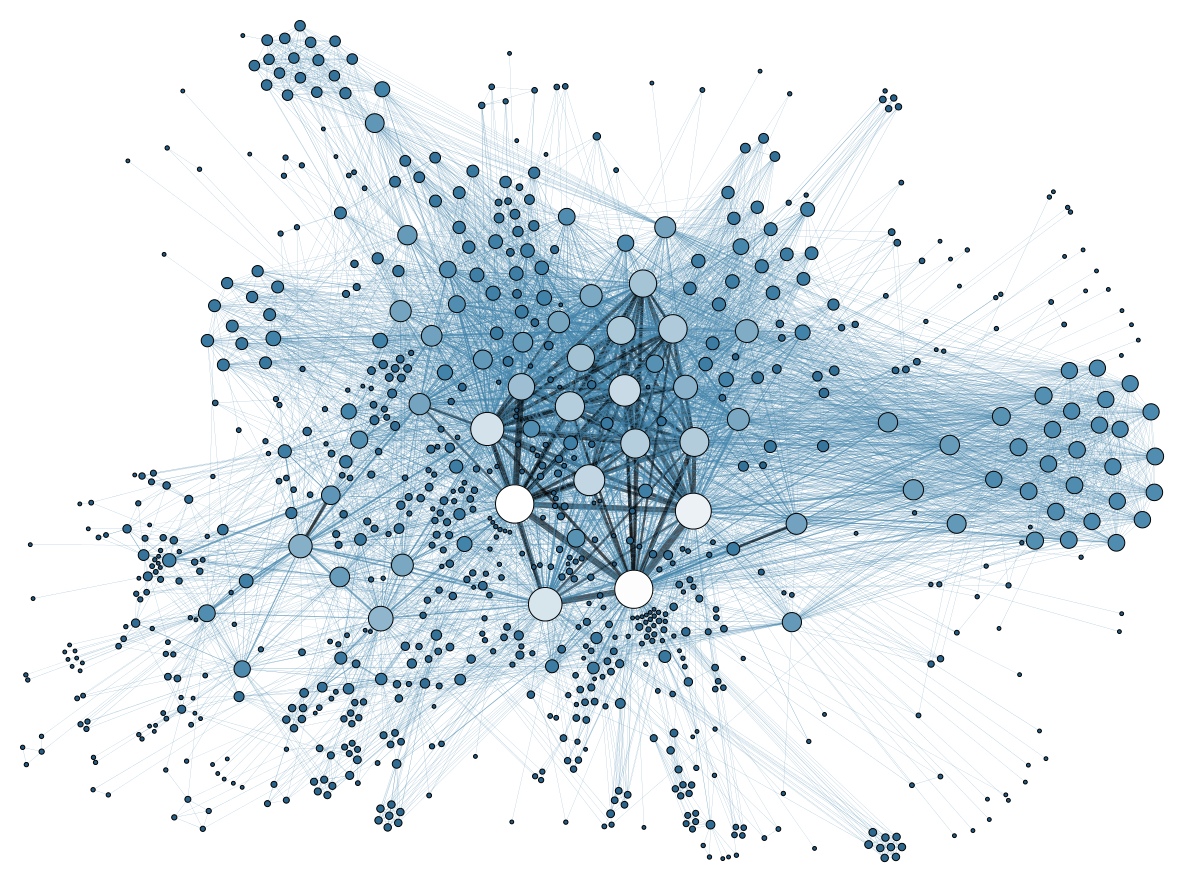
\includegraphics[width=7.8cm]{figures/fig2.png}
\end{center}
\caption{Nombre de la Figura.\cite{Mahmood2015}}
\label{figura1}
\end{figure}

\begin{figure}[H]
\centering
%\label{fig2}
\resizebox{6cm}{!} {
\begin{tikzpicture}%
   \begin{axis}[
      ylabel style={overlay},
      yticklabel style={overlay},
      xlabel={$x$},
      ylabel={$y$},
      legend style={at={(0.5,0.97)},
         anchor=north,legend columns=-1},
      domain=-2:2
   ]
   \addplot {x^2};
   \addplot {x^3};
   \addplot {x^4};
   \legend{$x^2$,$x^3$,$x^4$}
   \end{axis}
\end{tikzpicture}
}
\caption{El título}
\label{figura2}
\end{figure}

Tablas: Coloque las tablas al inicio o al final de las columnas. A diferencia de las figuras el título de las tablas se coloca en la parte superior de la misma. 
En la Tabla \ref{tabla1} de esta guía se muestra un ejemplo del formato para la presentación del artículo.
Debe verificar que igual que las figuras, las tablas que se encuentren en el artículo se citen en el texto principal. 

\begin{table}[H]
\centering
\captionof{table}{Tamaños de Fuente que se utilizan en la plantilla de articulos de la revista INGENIUS}
  \scalebox{0.74}{
    \begin{tabular}{cl}
    \toprule
    \multicolumn{1}{c}{Tamaño de letra} & \multicolumn{1}{c}{Uso} \\
    \midrule
    \small{10}    & \small{Datos del autor, título, texto de tablas y figuras.} \\
    {\textbf{12}} & \textbf{Resumen, palabras clave} \\
    12    & Nombre del autor(es), texto del artículo  \\
    \Large{13}    & \Large{Títulos de segundo y tercer orden} \\
    \LARGE{\textbf{15}} & \LARGE{\textbf{Títulos de primer nivel}} \\
    \huge{\textbf{18}} & \huge{\textbf{TITULO}} \\
    \bottomrule
    \end{tabular}%
}
  \label{tabla1}%
\end{table}

Ecuaciones: Utilice editor de ecuaciones desde OverLeaf.  Trate de que las ecuaciones sean compactas empleando en el signo (/), la función exponencial como exp, o subíndices y superíndices. Las ecuaciones requeridas dentro del modelo matemáticas serán enumeradas según se detalla a continuación en la Ec \ref{eq1}.

\begin{equation} 
\label{eq1}
\begin{array}{ll}
\alpha = \frac{l + s}{s} * \lambda & [veh]
\end{array}
\end{equation}

Unidades: Las unidades recomendadas son las del sistema métrico, en particular, se sugiere el uso del Sistema Internacional de Unidades (Unidades SI). Las unidades del sistema inglés pueden emplearse como unidades secundarias (en paréntesis). 

Abreviaturas: Se deben definir las abreviaturas y acrónimos que no sean comunes la primera vez que aparecen en el texto, aún si ya se han definido en el resumen. No utilice abreviaturas en el título a menos que sea inevitable.

\subsection{Referencias}

Se debe verificar con cuidado que todas las citas colocadas en el texto, aparezcan en la lista de referencias bibliográficas. En la lista solo deben aparecer las referencias que fueron utilizadas en el texto principal del trabajo, en las tablas o en las figuras, esto implica que no deben aparecer otras referencias aunque el autor las haya consultado durante la preparación del artículo.

        Las referencias incluidas en el texto se presentan al final ordenadas numéricamente en paréntesis cuadrados \cite{Valenzuela2019} según el orden de aparición en el texto. Un punto debe seguir al paréntesis \cite{Panwar2019}. Referencias múltiples pueden citarse con paréntesis separados por un guión \cite{Ramirez2015,Pagani2014,Peralta2017}. Cuando se cite un libro indicar las páginas con la información relevante. El título como tal de las “Referencias” al final del artículo no va numerado.
        
Puede consultar la guía del IEEE para la cita de referencias disponible en el link: \url{https://bit.ly/2PjrnJj}

Las referencias deben ser guardadas en el archivo \textbf{referencias.bib} en formato bibtex, indicando la \textbf{bibkey} secuencialmente según su aparición. Se recomienda utilizar un gestor bibliográfico para que pueda corregir previamente los metadatos como: autor, título, publisher, volume, issue, año, páginas, en caso de ser incorrectos \textbf{Mendeley}

\section{Resultados y Discusión}

Estos dos apartados suelen aparecer juntos en muchos trabajos. No se deben confundir esta discusión o análisis con la obtención de conclusiones, algo que depende tanto de los resultados y de su análisis como del marco teórico y de los objetivos.

El pseudocódigo de los algoritmos debe ser presentado según indica el ejemplo del algortimo

\begin{algorithm}[H]
\label{algo1}
\SetAlgoLined
\text{\textbf{Entrada:}} \text{Caso estudio}\\
\text{\textbf{Salida:}} \text{Global solución}\\
\KwResult{Escribir aquí el resultado }
 initialización\;
 \While{While condicion}{
  instructions\;
  \eIf{condición}{
   instrucciones1\;
   instrucciones2\;
   }{
   instrucciones3\;
  }
 }
 \caption{Como escribir algoritmos}
\end{algorithm}





%========================================================
\section{Conclusiones}

Las conclusiones deben obtenerse, por tanto, a partir de algo más que de los simples datos registrados. De hecho, unos datos o resultados pueden tener un sentido u otro y, por tanto, pueden llevar a unas conclusiones y otras, dependiendo del marco conceptual que justifica la investigación, de la metodología seguida, de los objetivos propuestos, etc.
%========================================================

\section*{Agradecimientos}
Este apartado es opcional que dependerá su utilización en caso de exister algun organismo financiador, colaborador, etc., que permitió llevar a cabo la investigación.
%========================================================


\bibliography{referencias.bib}
\bibliographystyle{IEEEtran}
\end{multicols}
\end{document}